%-----------------------------------------------------------------------------------------------------
%	INCLUSIÓN DE PAQUETES BÁSICOS
%-----------------------------------------------------------------------------------------------------
\documentclass[a4paper,12pt]{article}
%-----------------------------------------------------------------------------------------------------
%	SELECCIÓN DEL LENGUAJE
%-----------------------------------------------------------------------------------------------------
% Paquetes para adaptar Látex al Español:

%-----------------------------------------------------------------------------------------------------
%	SELECCIÓN DE LA FUENTE
%-----------------------------------------------------------------------------------------------------
% Fuente utilizada.
\usepackage{courier}                    % Fuente Courier.
\usepackage{microtype}                  % Mejora la letra final de cara al lector.
%-----------------------------------------------------------------------------------------------------
%	ALGORITMOS
%-----------------------------------------------------------------------------------------------------
\usepackage{algpseudocode}
\usepackage{algorithmicx}
\usepackage{algorithm}
\usepackage{listings}

%-----------------------------------------------------------------------------------------------------
%	IMÁGENES
%-----------------------------------------------------------------------------------------------------
\usepackage{float}
\usepackage{placeins}
%-----------------------------------------------------------------------------------------------------
%	ESTILO DE PÁGINA
%-----------------------------------------------------------------------------------------------------
% Paquetes para el diseño de página:
\usepackage{fancyhdr}               % Utilizado para hacer títulos propios.
\usepackage{lastpage}               % Referencia a la última página. Utilizado para el pie de página.
\usepackage{extramarks}             % Marcas extras. Utilizado en pie de página y cabecera.
\usepackage[parfill]{parskip}       % Crea una nueva línea entre párrafos.
\usepackage{geometry}               % Asigna la "geometría" de las páginas.
% Se elige el estilo fancy y márgenes de 3 centímetros.
\pagestyle{fancy}
\geometry{left=3cm,right=3cm,top=3cm,bottom=3cm,headheight=1cm,headsep=0.5cm} % Márgenes y cabecera.
% Se limpia la cabecera y el pie de página para poder rehacerlos luego.
\fancyhf{}
% Espacios en el documento:
\linespread{1.1}                        % Espacio entre líneas.
\setlength\parindent{0pt}               % Selecciona la indentación para cada inicio de párrafo.
% Cabecera del documento. Se ajusta la línea de la cabecera.
\renewcommand\headrule{
	\begin{minipage}{1\textwidth}
	    \hrule width \hsize
	\end{minipage}
}
% Texto de la cabecera:
\lhead{\subject}                          % Parte izquierda.
\chead{}                                    % Centro.
\rhead{\doctitle \ - \docsubtitle}              % Parte derecha.
% Pie de página del documento. Se ajusta la línea del pie de página.
\renewcommand\footrule{
\begin{minipage}{1\textwidth}
    \hrule width \hsize
\end{minipage}\par
}
\lfoot{}                                                 % Parte izquierda.
\cfoot{}                                                 % Centro.
\rfoot{Page\ \thepage\ of\ \protect\pageref{LastPage}} % Parte derecha.


%----------------------------------------------------------------------------------------
%   MATEMÁTICAS
%----------------------------------------------------------------------------------------

% Paquetes para matemáticas:
\usepackage{amsmath, amsthm, amssymb, amsfonts, amscd} % Teoremas, fuentes y símbolos.
\usepackage{dsfont} % new fonts added by contributors
\usepackage{tikz-cd} % para diagramas conmutativos
\usepackage[mathscr]{euscript}
\let\euscr\mathscr \let\mathscr\relax% just so we can load this and rsfs
\usepackage[scr]{rsfso}
\newcommand{\powerset}{\raisebox{.15\baselineskip}{\Large\ensuremath{\wp}}}
 % Nuevo estilo para definiciones
\usepackage{hyperref}

%-----------------------------------------------------------------------------------------------------
%	BIBLIOGRAFÍA
%-----------------------------------------------------------------------------------------------------

\usepackage[backend=bibtex, style=numeric]{biblatex}
\usepackage{csquotes}

\addbibresource{references.bib}

%-----------------------------------------------------------------------------------------------------
%	PORTADA
%-----------------------------------------------------------------------------------------------------
% Elija uno de los siguientes formatos.
% No olvide incluir los archivos .sty asociados en el directorio del documento.
%\usepackage{title1}
\usepackage{title2}
%\usepackage{title3}

%-----------------------------------------------------------------------------------------------------
%	TÍTULO, AUTOR Y OTROS DATOS DEL DOCUMENTO
%-----------------------------------------------------------------------------------------------------

% Título del documento.
\newcommand{\doctitle}{The Group Law for Edwards Curves}
% Subtítulo.
\newcommand{\docsubtitle}{}
% Fecha.
\newcommand{\docdate}{}
% Asignatura.
\newcommand{\subject}{}
% Autor.
\newcommand{\docauthor}{Rodrigo Raya Castellano}
\newcommand{\docaddress}{Technical University of Munich}
\newcommand{\docemail}{}

%-----------------------------------------------------------------------------------------------------
%	RESUMEN
%-----------------------------------------------------------------------------------------------------

% Resumen del documento. Va en la portada.
% Puedes también dejarlo vacío, en cuyo caso no aparece en la portada.
%\newcommand{\docabstract}{}
\newcommand{\docabstract}{}

\begin{document}

\makeatletter\renewcommand{\ALG@name}{Algoritmo}

\maketitle

%-----------------------------------------------------------------------------------------------------
%	ÍNDICE
%-----------------------------------------------------------------------------------------------------

% Profundidad del Índice:
%\setcounter{tocdepth}{1}

\newpage
\tableofcontents
\newpage

\section{Introduction}
The development of formal proofs of the group law of elliptic curves is very old. However, most of the works we are aware of focus on the group law for elliptic curves in Weierstrass form. Proofs varied largely on the theoretical complexity of the arguments used. For instance, in \cite{bartzia2014formal}, the authors develop a formal library for elliptic curves and the group law is shown establishing an isomorphism between the elliptic curve and its Picard group of divisors. Simpler arguments exist. For instance, \cite{thery2007proving} provides a more practical approach based on computationally intensive reasoning techniques rather than in sophisticated mathematical concepts. Here the author already points out one of the main challenges that elliptic curve verification presents to a modern theorem prover: 

\begin{displayquote}
To translate this 7 page long paper proof in a theorem prover was a real challenge. In fact, the proof relies on some non-trivial computations that the author advises to check using a computer algebra system such as CoCoA. The main difficulty has been to find an effective way to cope with these computations inside our proof system. 
\end{displayquote}

The author of this report conducted a similar case study two years ago \cite{techreport} following closely \cite{russinoff2017computationally}. This experience made him realise that the problem of verifying elliptic curves was not trivial at all and in fact, constitutes an ideal experiment to test the health of a theorem prover since it is both simple to understand and difficult to implement. Far are the times in which some textbooks could summarise the question as follows \cite{silverman1992rational}:

\begin{displayquote}
Of course, there are an awful lot of special cases to consider, such as when one of the points is the negative of the other or two of the points coincide. But in a few days you will be able to check associativity using these formulas. So we need say nothing more about the proof of the associative law!
\end{displayquote}

There is already an entry on the Archive of Formal Proofs that formalizes elliptic curves in Weierstrass form \cite{Elliptic_Curves_Group_Law-AFP}. Nevertheless, there is much less work done on elliptic curves in Edwards form. This can be explained by their relative novelty as they were first proposed in 2007 by Harold Edwards \cite{edwards2007normal}. 

Despite this, we find a similar situation to that encountered with Weierstrass curves. On the one hand, there exist proofs whose mathematical content is quite deep. For instance,  Edwards himself proposed an approach based on differential equations in connection with previous work by Euler and Gauss. Another approach is to build a so called rational equivalence between curves in Edwards form and curves in Weierstrass form \cite{das2008pairing} and then transfer the group properties from one to the other. A more practical approach has more recently been proposed and partially mechanized by Hales \cite{edwards2007normal}. In the present work, this last approach was followed.

\pagebreak
\section{Edwards curves}
\subsection{Affine Edwards curves}

Let $k$ be an arbitrary field (for simplicity we assumed $k = \mathbb{R}$ in our proof). We define an Edward curve $E$ as the set of zeros of the following multivariate polynomial:

$$e(x,y) = x^2 + cy^2 - 1 - d x^2y^2$$

where $c,d,x,y \in k$ and $c,d$ are fixed. Then one defines the addition of two points on the curve as:

$$z_1 \oplus z_2 = (x_1,y_1) \oplus (x_2,y_2) = \Big(\frac{x_1x_2-cy_1y_2}{1-dx_1x_2y_1y_1},\frac{x_1y_2+y_1 y_2}{1+d x_1 x_2 y_1y_2}\Big)$$

The motivation for this addition is explained in \cite{hales2016group} in a very accessible manner without going into the details of algebraic geometry. Essentially, one reinterprets the normal complex multiplication:

$$(x_1,y_1) \cdot (x_2,y_2) = (x_1 x_2 - y_1 y_2, x_1 y_2 + x_2 y_1)$$

by considering the family of hyperbolas in the plane that pass through $z = (-1,0)$ and whose asymptotes are parallel to the coordinate axes, these are given by the equation:

$$xy + p(x + 1) + qy = 0$$

Every two points $z_1$ and $z_2$ on the circle intersect some hyperbola within the family. The hyperbola meets the unit circle in one additional point $z_3$:

\begin{center}
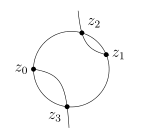
\includegraphics{img/hyp_circ.png}
\end{center}

It turns out that $z_1 z_2 z_3 = 1$ and one may define complex multiplication as $z_1 z_2 = \overline{z_3}$. The very same construction works for general elliptic curves and gives the addition formula above:

\begin{center}
	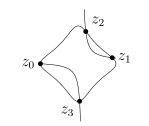
\includegraphics{img/hyp_ellip.png}
\end{center}

The goal of \cite{hales2016group} is to show that $(E,\oplus)$ is an abelian group. This is only feasible for affine Edwards curves when $d$ is not a non-null square.

\subsection{Projective Edwards curves}

Introduced to bypass the restriction that $d$ should not be a non-null square. 

Introduced by gluing two affine curves $E_{\text{aff}}$ together. 

The associative property for $E$ is a direct consequence of the associative property of the affine pieces $E_{\text{aff}}$.

More formally, one introduces the set $E_{\text{aff}}$ as the set of zeros of the equation:

$$e(x,y) = x^2 + y^2 - 1 - t^2 x^2 y^2$$

One also denotes by $E_{\text{circ}}$ the subset $E_{\text{aff}}$ whose coordinates $x,y$ are non-zero. Finally, in the cartesian product $E_{\text{aff}} \times E_{\text{aff}}$ we use the notation $(P,i)$ to refer to point $P$ of $E$ using the $i$-th copy of $E_{\text{aff}}$ and we identify over the elements of $E_{\text{circ}}$ the pair of points $(P,i)$ and $(\tau P, i+1)$. So elements of $E$ are actually classes of points that we denote by $[P,i]$.

The addition on $E$ requires first to define a second addition $\oplus_1$ (previous addition is denoted from now on by $\oplus_0$) given by:

$$z_1 \oplus_1 z_2 = (x_1,y_1) \oplus_1 (x_2,y_2) = \Big(\frac{x_1y_1-x_2y_2}{x_2y_1 - x_1y_2},\frac{x_1y_1+x_2 y_2}{x_1 x_2 + y_1y_2}\Big)$$

Finally, addition on $E$ is defined by:

$$[P,i] \oplus [Q,j] = [P \oplus_l Q, i+j]$$

if $\delta_l(P,Q) \neq 0, l \in \mathbb{F}_2 = \{0,1\}$ where $\delta_l$ is the magnitude ensuring that the quotients are non-zero. Here, one still needs to prove that $\oplus$ is well-defined. Well-definition and an auxiliary lemma called dichotomy are actually the hardest properties to be established in the development. 

\subsection{Use of Edwards curves}

Edwards curves present several advantages compared to traditional Weierstrass form. To start with, they lead to an explicit formula for addition while in Weierstrass curves addition needs to take care of the special \textit{infinity point}. Also, Bernstein and Lange \cite{bernstein2007faster} showed that addition and multiplication by scalars could be done more efficiently over these curves. Another strong property noted in this study is that if $d$ is not a square the addition was defined for all input pairs on the curve. This is the so-called completeness property of addition. Essentially, it tells that the Edwards addition law can carry out any sequence of group operations, without risk of failure \cite{bernstein2007faster}.

Furthermore, there are important issues arising from the implementation of elliptic curves that should be kept in mind. Literature has given special attention to the so-called side-channel attacks. These cryptographic attacks are based in the measurement of the physical parameters of the system. For instance, one could measure the power consumption \cite{kocher1999differential} or the time spent in executing the underlying algorithm \cite{kasper2011fast} in order to gain information on the cryptographic parameters used. Edwards curves seem to be useful to prevent this kind of attacks \cite{bernstein2007faster}.  

As for projective Edwards curves, which are known in the literature as twisted Edwards curves, they provide a generalization of affine Edwards curves covering a wider range of algebraic curves (in particular, the important class of Montgomery curves) which leads to faster arithmetic computations. The advantage of formalizing this curves lies in the fact that we do not special conditions on the defining parameters to get a group law with their addition \cite{bernstein2008twisted}. 


All of these properties made Edwards curves and their extensions to be of interest in the field of elliptic curve cryptography. 




\pagebreak
\section{Isabelle tools used}
\subsection{The use of locales}

During this project, I had a first contact with the tools that Isabelle uses to manage theories. These are not normally introduced in a basic course on the proof assistant and we had to explore on our own using the existing documentation \cite{ballarin2010tutorial}. We worked both with external locales (such as comm\_group):

\begin{figure}[!htbp]
	\centering
	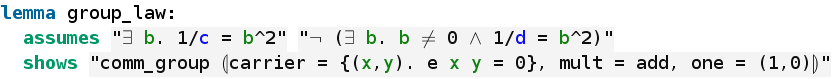
\includegraphics[width=\linewidth,height=\textheight,keepaspectratio]{img/group_law.png}
	\caption{The group law theorem for affine elliptic curves using comm\_group locale}
	\label{fig:grouplaw}
\end{figure}

and our own locales that served to structure and particularize the theories:

\begin{figure}[!htbp]
	\centering
	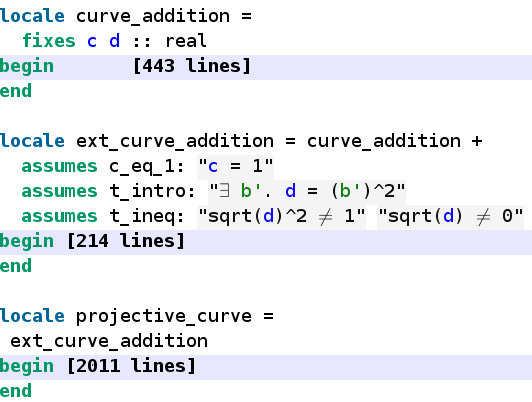
\includegraphics[width=0.8\linewidth,height=0.8\textheight,keepaspectratio]{img/structure.png}
	\caption{General structure of the theory organized in locales}
	\label{fig:grouplaw}
\end{figure}
	
\subsection{The algebra method}

A good understanding of the proving tools at our disposal can save a lot of work. The algebra method \cite{wenzel2019isabelle} has as one of its basic functionalities solving the following quantified formula: 

\begin{align*}
\forall x_1 \ldots x_n. &  \\        
& e_1(x_1,\ldots,x_n) = 0 \land \ldots \land e_m(x_1,\ldots,x_n) = 0 \to \\
& (\exists y_1, \ldots, y_k. \\
& p_{11}(x_1,\ldots,x_n) y_1 + \ldots + p_{1k}(x_1,\ldots,x_n) y_k = 0 \land \\
& \ldots \land \\
& p_{t1}(x_1,\ldots,x_n) y_1 + \ldots + p_{tk}(x_1,\ldots,x_n) y_k = 0) \\
&
\end{align*}

where $e_1,\ldots,e_n$ and $p_{ij}$ are multivariate polynomials in the indicated variables. In our case, $e_i$ could be the hypothesis that we have certain point in the curve and the exists fragment corresponds to the search of division quotients. As a direct consequence, one does not always need to copy the polynomial quotients obtained with Mathematica. Here is an example:

\begin{figure}[!htbp]
	\centering
	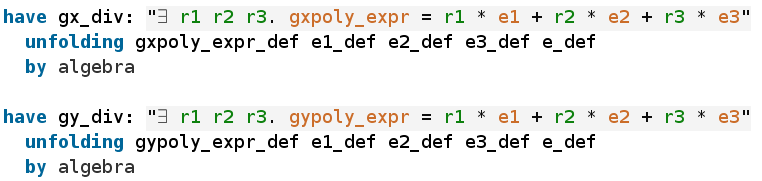
\includegraphics[width=0.8\linewidth,height=0.8\textheight,keepaspectratio]{img/poly_expr.png}
	\caption{Example of polynomial division with the algebra method}
	\label{fig:groebner}
\end{figure}

The variables gxpoly\_expr, gypoly\_expr correspond to given polynomials that are computed explicitly with Mathematica. However, in our case, there is no need to copy the expressions for $r1,r2,r3$ since all we need is their existence. This is in contrast to the situation found in \cite{hales2016group}

\subsection{The use of Gröbner basis}

Hales explicitly uses Gröbner basis to go through the proof of dichotomy. This property is fundamental to establish the well-definition of the group law for projective Edwards curves. To be precise, it would be need in Isabelle whether a given set of polynomials corresponds to a Gröbner basis of a given polynomial ideal. However, the representation of this theory is quite different to ours:

\textit{Essentially, polynomials are represented as ordered lists of monomials, where monomials are represented as pairs consisting of a coefficient and a power-product (I.e., something like $x_0*y_0$); power-products are represented similarly, as ordered lists of indeterminate-exponent-pairs. Indeterminates, finally, are typically represented by natural numbers (although this can be changed easily). See also \cite{maletzky2018grobner}.}

While in practice the computation of Gröbner basis in Isabelle might look like in Figure \ref{fig:groebner}.

\begin{figure}[!htbp]
	\centering
	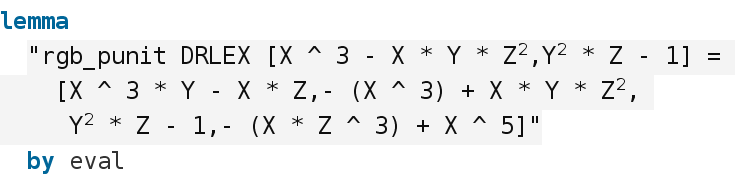
\includegraphics[width=0.8\linewidth,height=0.8\textheight,keepaspectratio]{img/groebner.png}
    \caption{Gröbner basis computation in Reduced\_GB\_Examples.thy}
    \label{fig:groebner}
\end{figure}

more expertise on this theory would be needed in order to connect it with our own. This can be considered as future work since having at our disposal an easy access to verified Gröbner basis computation would have speeded the proof process significantly. 

On the other hand, the algebra method is not capable to solve this problem either. While it computes Gröbner basis for the purpose of proving whether a polynomial is in the generated ideal, this computation is done outside the logic. In particular, it is not proved that the computed basis is indeed a Gröbner basis. 

As a last alternative, one could check by hand that the involved identities hold. This is what Hales suggests in the article when he says: \textit{In particular, our approach does not require the use of Gröbner bases (except in Lemma 4.3.2 where they make an easily avoidable appearance)}. 

Here is one example of such a hand computation. We follow the notation in \cite{hales2016group}. Namely, we focus on equation 19:

$$(x_0^2 - x_1^2,y_0^2 - x_1^2,x_0y_0 - x_1 y_1) \equiv (0,0,0) \; mod \; S_{\pm}$$

where $S_{\pm}$ is the Gröbner basis associated with certain polynomials known to evaluate to zero. One then deduces one by one the corresponding equations:

To start, one deduces the third equality:

$$\delta' = x_0 y_0 \delta_{0x} x_1 y_1 \Big(\frac{1}{t x_0}\Big) \Big(\frac{1}{t y_0}\Big) = 
x_0 y_0 \Big(1 - \frac{t^2 x_1 y_1}{t^2 x_0 y_0}\Big) = x_0y_0 - x_1 y_1$$

Since by assumption $\delta_{-} = 0$ we have the third equality and we note:

$$(1) \; x_0 = x_1 \Big(\frac{y_1}{y_0}\Big)$$

where we have that $x_0,y_0,x_1,y_1 \neq 0$.

For the second, we have:

$$\delta_{+} = t x_0 t_0 \delta_{1x} x_1 y_1 \Big(\frac{1}{tx_0}\Big) \Big(\frac{1}{ty_0}\Big) = t x_0 y_0 \Big(\frac{y_1}{t x_0} - \frac{x_1}{t y_0}\Big) = y_0 y_1 - x_0 x_1 \stackrel{1}{=} y_0 y_1 - x_1^2 \Big(\frac{y_1}{y_0}\Big) = \frac{y_1}{y_0} (y_0^2 - x_1^2)$$

since $\delta',\delta_{+} = 0$, we have the second equation. We also note: 

$$(2) \; \frac{y_1}{y_0} (y_0^2 - x_1^2) = 0$$

Finally, the third equation is obtained as follows:

$$x_0^2 - y_1^2 \stackrel{1}{=} x_1^2 \frac{y_1^2}{y_0^2} - y_1^2 = \Big(\frac{y_1^2}{y_0^2}\Big) (x_1^2 - y_0^2) \stackrel{2}{=} \frac{y_1^2}{y_0^2} (x_1^2 - y_0^2) \stackrel{2}{=} 0$$

One should note that not all the polynomials of $S_{\pm}$ were used in this deduction.

\subsection{The representation of projective elliptic curves}

We have discussed the representation of projective Edwards curves as described in \cite{hales2016group}. The challenge to represent this description is similar to the representation of equivalence classes in \cite{paulson2006defining}. Here is, to start with, the definition of projective addition:

\begin{figure}[!htbp]
	\centering
	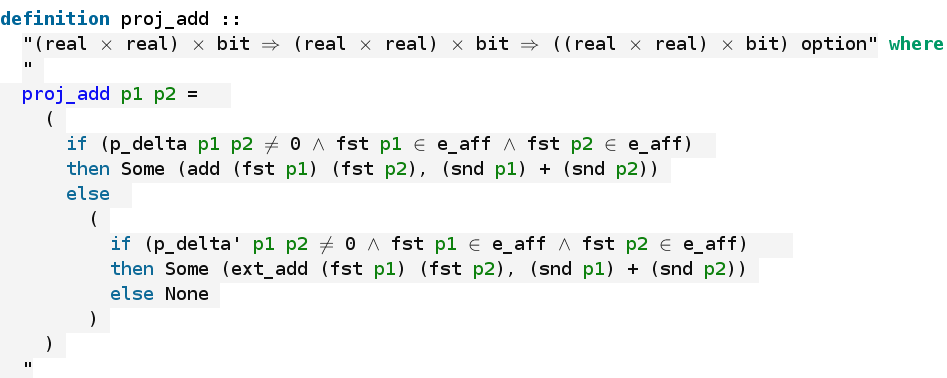
\includegraphics[width=\linewidth,height=\textheight,keepaspectratio]{img/proj_add.png}
	\caption{Projective addition on points}
	\label{fig:proj_add}
\end{figure}

A posteriori, one notes that it would be more convenient to have a more balanced definition without the if-else construct. The version in figure \ref{proj_add_domain} would save some work. For instance, to show that we are in the second branch of the if, we would not need to show that the first branch has a false guard.

\begin{figure}[!htbp]
	\centering
	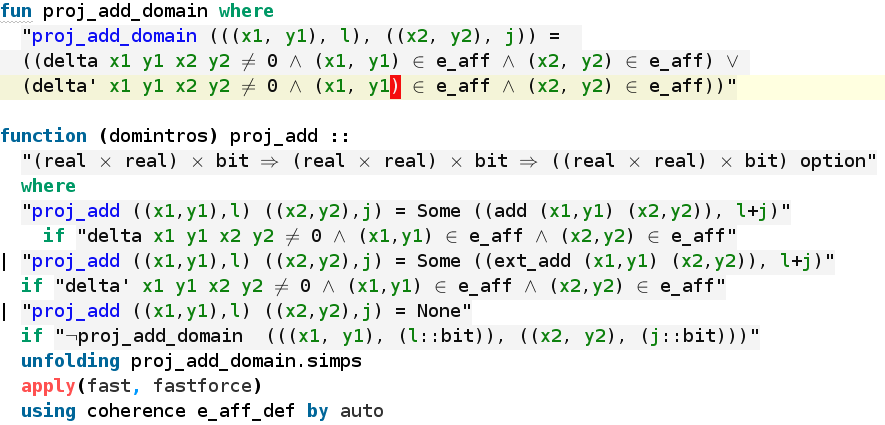
\includegraphics[width=\linewidth,height=\textheight,keepaspectratio]{img/proj_add_domain.png}
	\caption{Balanced version of the projective addition on points}
	\label{fig:proj_add_domain}
\end{figure}

Before introducing proper projective addition, we introduce how are projective points represented:

\begin{figure}[!htbp]
	\centering
	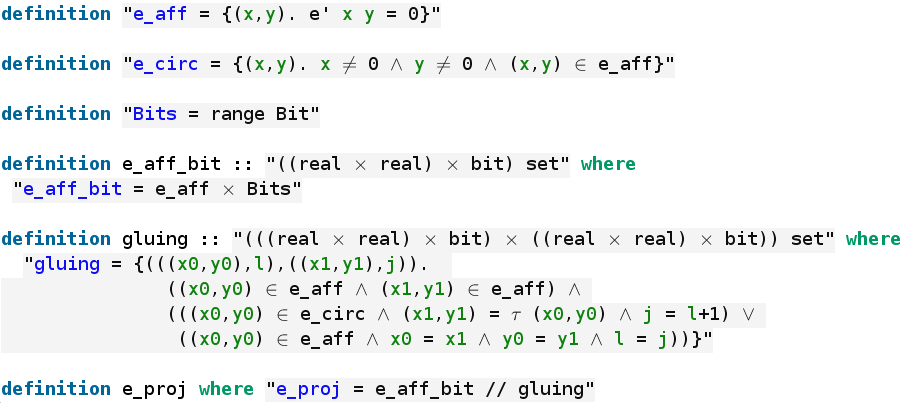
\includegraphics[width=\linewidth,height=\textheight,keepaspectratio]{img/e_proj.png}
	\caption{Projective points representation}
	\label{fig:e_proj}
\end{figure}

So points that satisfy the equation given by $e'$ an which are non-zero are identified with their inversions modulo $\tau$. The other conditions in the equivalence relation only ensure the reflexivity property. It is on these classes of points that projective addition should work. Figure \ref{fig:proj_add_class} shows the adaption of proj\_add to classes. 

proj\_add\_class first selects those pairs that lead to some result, then it actually computes the result and finally identifies equivalent points. Much later, when we prove covering and well-definition we show that indeed the last identification provides only one class. This is the class that is selected with the\_elem in proj\_addition.

\begin{figure}[!h]
	\centering
	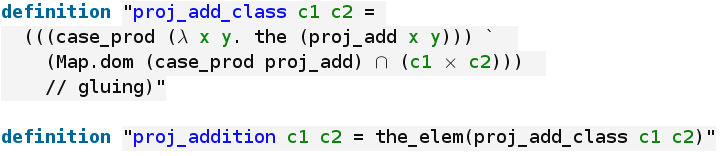
\includegraphics[width=\linewidth,height=\textheight,keepaspectratio]{img/proj_add_class.png}
	\caption{Projective addition on classes of points}
	\label{fig:proj_add_class}
\end{figure}









\pagebreak
\section{Notes on the proof}
The proof is maintained on Github at \href{https://github.com/rjraya/Isabelle/blob/master/curves/Hales.thy}{this repository}.

Once loaded in the editor, there are three sections. The first section formalises the plain affine elliptic curve group law. Second and third sections are dedicated to the projective group addition. The second section formalises the main preliminaries and the third formalises the group law properties of the addition for projective Edwards curves. The theorems and lemmas follow closely the nomenclature from \cite{hales2016group} and in a definitive version the corresponding numbering will be added to make it clearer. 

The current state of the proof is as follows: we formalised the paper until page 14 where we had to stop since we could not compute the required Gröbner basis. Instead, some of the hand computations that were described in previous sections were implemented, but there remain some to be completed. This would essentially finish dichotomy. Lemmas 4.3.3 and 4.3.4 were also fully formalised. Finally, from theorem 4.4.1, which establishes the group law of projective Edwards curves, it would remain to finish the proofs of associativity and closure. These follow similar techniques to the ones shown previously.

Pages 17-20, develop alternative proofs of previous theorems and formalise facts appearing in the motivation. There are no formalisations/Mathematica computations for this section in the original paper. Overall, we think that the full formalisation should contain the material presented until page 16 and that the last section is less important for practical purposes.




\pagebreak
\section{Conclusions}
During the spring semester of 2017, I worked in developing a proof of the group law of Weierstrass elliptic curves. The system at hand was called Welder and allowed the user to reason with the basic rules of natural deduction. There were no tactics or any specialized tools to assist in proving. As it may be understood we did not go very far in our formalisation. We formalised part of the basics theorems about field theory and some of the basic proofs of the group law of the corresponding curve.

On the other hand, the pedagogical benefit of this experience can be hardly contested. We learnt that theorem proving is hard (too hard indeed). However, at the same time we did experiment the joy of problem solving. Nowadays, the mathematics student is surrounded with such a great quantity of information and materials that he can find solutions to his problems without thinking the solution by himself. He can also mistake wrong proofs for right ones without noticing. Theorem proving solves this by focusing the attention of the student. Otherwise work would not progress. I believe this is a valuable virtue of theorem proving.

A second benefit of this experience was that I was forced to do research on the methodologies that existed in order to improve the proving experience. I spent the summer holidays of 2017 reading the book Term rewriting and all that \cite{baader1999term}. It was this experience which ultimately encouraged me to come to the Technical University of Munich and learn Isabelle. 

If I learnt something during my experience with Welder was that proving correct the group law of an elliptic curve was a great benchmark to test the health of a proving engine. In much less time, Isabelle let me prove the group law of a large class of affine elliptic curves. We did actually prove more than what was made in the original paper by Hales, since we did not just verify the polynomials identities obtained through the proof but we did show the complete proving process. 

On the section of projective curves, while we did find a lot more difficulties, these reduced to the use of particular theories and techniques of proving in the system. It should be noted that these proofs were not formalised at all in previous work and the only existing certificate was the Mathematica computations provided. I believe that with sufficient cooperation between the different researchers we have been in contact to, it should not take much development time to finish all the details. 

Future work could tackle the implementation of algorithms for elliptic curve cryptography in Isabelle/HOL. Apparently, this was a student project proposal at the Chair of Software Reliability and Theoretical Computer Science which was never assigned. For this purpose, it could also be interesting to formalise the Montgomery family of elliptic curves since their combination with Edwards curves has been proposed to provide more robust implementations  \cite{costello2018montgomery}.








\pagebreak


\printbibliography

\end{document}